
\begin{frame}{Impact du numérique}{Origine}
%--	\begin{figure}[h!]

\begin{block}{Fabrication à partir de ressources naturelles}
\begin{figure}[h!]

\begin{minipage}[b]{0.5\linewidth}
Les minerais rares
\begin{itemize}
    \item Bismuth
    \item Cobalt
    \item Germanium
    \item Silicium
    \item Tantale
    \item Prométhéum
\end{itemize}

\end{minipage}\hfill
\begin{minipage}[b]{0.45\linewidth}  
\begin{figure}
    \centering
    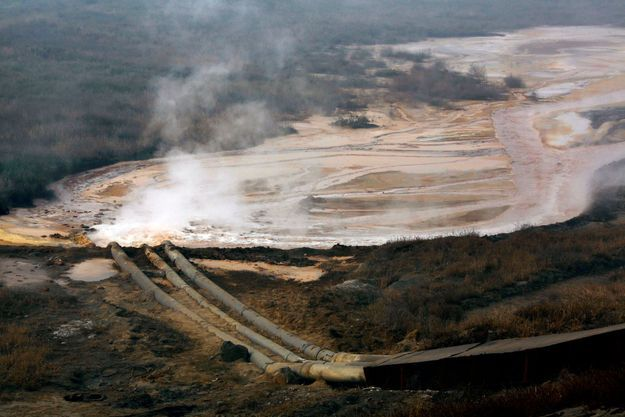
\includegraphics[scale=0.17]{Feathergraphics/lac.jpg}
    \caption{Lac de Baotou}
\end{figure}
\end{minipage}\hfill


\end{figure}

\end{block}
\begin{block}{Utilisation et destruction }
    
\begin{figure}[h!]
\begin{minipage}[b]{0.27\linewidth}
 $\nearrow$ Energie produite
\begin{figure}
    \centering
    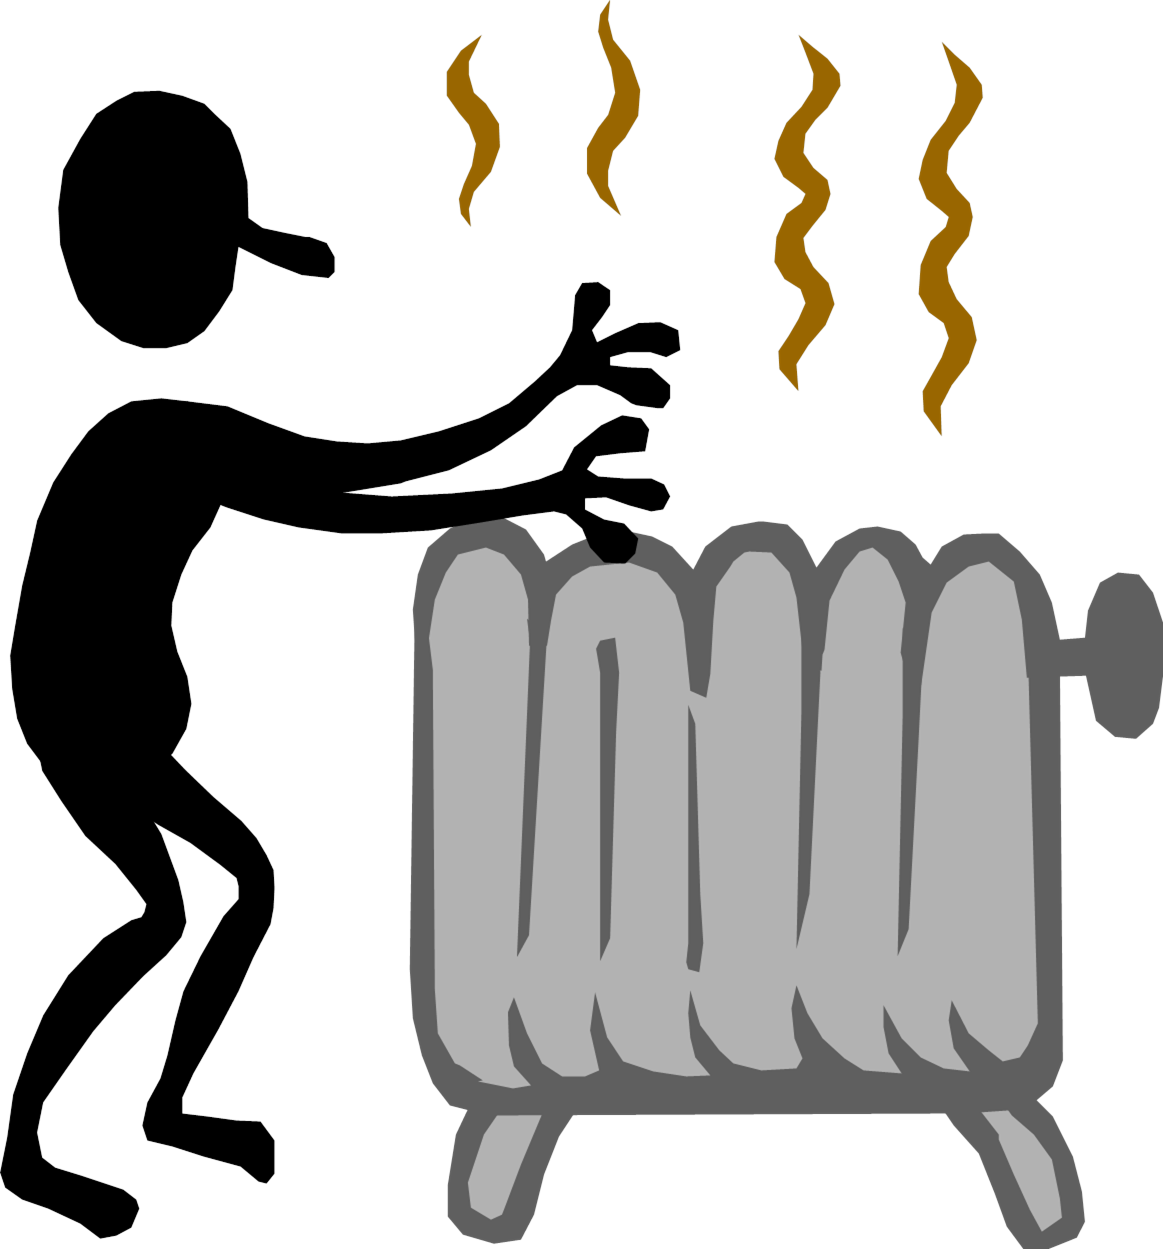
\includegraphics[scale=0.26]{Feathergraphics/rad.png}
\end{figure}
\end{minipage}\hfill
\begin{minipage}[b]{0.3\linewidth}  
4000 Data Centers

\begin{figure}
    \centering
    
\includegraphics[scale=0.03]{Feathergraphics/ville.png}
\end{figure}
\end{minipage}\hfill
\begin{minipage}[b]{0.3\linewidth}  
$5\%$ recyclés

\begin{figure}
    \centering
    
\includegraphics[scale=0.06]{Feathergraphics/poubelle.png}
\end{figure}
\end{minipage}
\end{figure}

\end{block}


\end{frame}
